\section{Introduction}
\label{section:intro}

% \textbf{Paragraph Goal: Establish the broad technological context, highlighting the tension between increasing capability and rising resource costs.}
% \textbf{Domain} built on \textbf{Foundational Technology} \citep{cite1} continue to advance in \textbf{Capability}, with \textbf{Trend Analysis} showing systematic improvements as \textbf{Scale/Complexity} increases \citep{cite2}. Yet this growth also amplifies \textbf{Problem} \citep{cite3}, making \textbf{Problem} a \textbf{Wider problem impact}.

% \textbf{Paragraph Goal: Explain the domain gap (e.g memory efficient) and how the current domain and hos solutions that solve this gap (e.g distillation, quantization)}

% \textbf{Paragraph Goal: Here you define, base and explain the Gap and the pain of the gap that existing in the previous approaches, its have to be the main things we addressing in this work.}

% \textbf{Paragraph Goal: Introduce the key scientific insight or "clue" from related literature that suggests a smarter way to solve the problem (e.g., signal sparsity). }
% Concurrently, \textbf{Related Field} studies show that \textbf{fact} can  \textbf{do something that intuitionally can cover the other work gap}, such as \textbf{Property X} and \textbf{Property Y} \citep{cite10}, and further indicate that \textbf{fact} concentrate in \textbf{Specific Similar Areas} \citep{cite11}. This evidence motivates using \textbf{the fact } to drive \textbf{ the domain of this work as well, should be what our method actully doing } \citep{cite12}.

% \textbf{Paragraph Goal: Critique the status quo by explaining how current standard methods fail to utilize the insight mentioned above (i.e., they are context-agnostic). }
% In contrast, prevailing \textbf{Existing Frameworks} are \textbf{Context-Agnostic}: they optimize \textbf{Local Metrics}—such as \textbf{Metric A}, \textbf{Metric B}, or \textbf{Metric C}—rather than \textbf{End-Task Performance} \citep{cite13}. Consequently, \textbf{Resources} are often assigned using \textbf{Uniform/Heuristic Schemes} that ignore \textbf{Contextual Importance}, rather than prioritizing \textbf{Critical Components}. This design can \textbf{Lead to Inefficiency} and \textbf{Suboptimal Performance}, and it typically omits objectives that preserve \textbf{Critical Features} during \textbf{Transformation Process} \citep{cite14}.

% \begin{figure}[H]
    \centering
  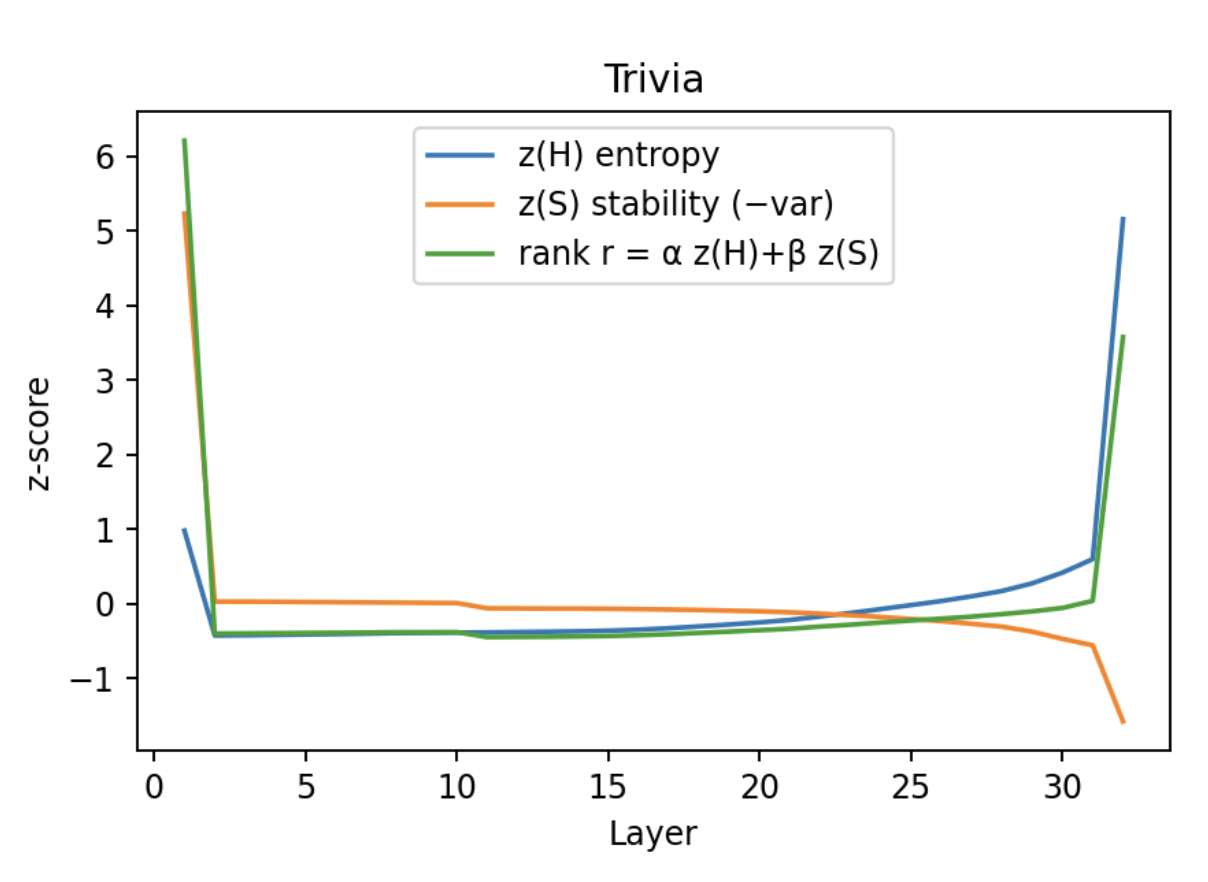
\includegraphics[width=1\linewidth]{imgs/teaser_fig.png}
  \caption{Teaser Fig Explain the phenomena.}
    \label{fig:bbq_full}
\end{figure}
% \label{tesear}


% \textbf{Paragraph Goal: Formally propose the new method(s), explaining how they bridge the gap by directly applying the insight to the problem  gap.} 
% In this work, we ask whether \textbf{Leveraging the phenomena} can guide \textbf{Your Focus Area}. Unlike prevailing \textbf{Existing Frameworks}, which are \textbf{agnostic of this phenomena} and rely on \textbf{Proxy Objectives}, we propose \textbf{Method Name (Acronym)} that leverage \textbf{ the phenomena} into \textbf{The method } as we empathizes at \ref{tesear} \textbf{explain the fig} . Concretely, \textbf{Acronym} computes \textbf{Relevance Scores} from \textbf{Data Source} on a \textbf{dataset}, then solves a \textbf{Constraint Problem} that assigns \textbf{Higher Resources} to the most \textbf{Relevant Components} while aggressively \textbf{Reducing Resources} elsewhere. 


% \textbf{Paragraph Goal: Summarize the core technical contributions and key empirical findings, three points of contribution.}
% Our contributions are: \begin{itemize} \item \textbf{Method Name:} a \textbf{Framework Type} that derives \textbf{Component Relevance} from \textbf{phenomena} and  \textbf{doing the something much better}. \item \textbf{another thing}. \item \textbf{Empirical results:} across \textbf{Benchmarks} on \textbf{Systems}, \textbf{Acronym} maintains \textbf{Performance Metric} within \textbf{Delta} of \textbf{Upper Bound} while reducing \textbf{Cost Metric}. \end{itemize}

% %Paragraph Goal: Outline the organizational structure of the remainder of the paper. 
% The remainder of this paper is organized as follows. \S\ref{back} reviews \textbf{Background Area 1}, \textbf{Background Area 2}, and related background. \S\ref{method} introduces \textbf{Acronym}, its motivation, and the \textbf{Technical Implementation}. \S\ref{Experiments} reports experimental results. Finally, \S\ref{sec:discussion} discusses implications, limitations, and future directions.